\section{Initialisation de la connexion}
\subsection{En-têtes des trames}
\paragraph{}
Voyons tout d'abord le squelette d'une trame. Pour commencer, une trame envoyée ne contient pas juste une en-tête SSH et ses données. Elle contient d'abord une en-tête Ethernet, puis une en-tête IP ainsi qu'une en-tête TCP, correspondant respectivement à des protocoles ou des couches du modèle OSI liaison, réseau, transport et application. \cite{cadegros_etude_2023}

\begin{leftbar}
    \emph{Le modèle OSI}, défini en 1978, est un ensemble de normes permettant à des équipements réseau de communiquer entre eux de manière fiable, au travers de différents protocoles. Le modèle est basé sur le fait qu'une communication peut se découper en plusieurs sous-étapes contenues dans différentes couches, au total 7, allant du plus bas niveau (couche physique) vers le plus haut niveau (couche application). Lors de l'émission d'une trame, on retrouve plusieurs protocoles, correspondantes aux différentes couches, encapsulées les unes dans les autres. Toutes les couches ne sont pas forcément représentée, comme c'est le cas ici. \cite{gerossier_cours_2020}
\end{leftbar}

On retrouve en premier une trame du protocole Ethernet, qui ne contient que les adresses MAC source et destination, ainsi que le protocole de la couche suivante, ici IPv4. Cette partie sert à orienter une trame dans un réseau local et sera modifiée en cas de changement de réseau par un routeur.
L'en-tête IPv4, contient entre autres les adresses IP des deux machines (client et serveur), ainsi que, là encore, le protocole de la couche suivante, TCP.
Ce dernier, contient pour ce qui nous intéresse, les ports source et destination, ainsi que les numéros de séquences et d'acquittement, permettant une fiabilisation des échanges. \cite{cadegros_etude_2023}

\begin{leftbar}
    \emph{Le protocole TCP} permet d'établir une connexion fiable avec une machine distante, avec des phases d'initialisation et de clôture de la connexion. Cela permet alors un mode \og connecté \fg. Une connexion se déroule ainsi: le client envoie une séquence de synchronisation, auquel le serveur répond par une acceptation. Enfin, le client acquitte cette réponse. La fiabilité des échanges est assurée par un système d'accusé de réception, se basant sur les numéros de séquence et d'acquittement contenus dans les trames. \cite{gerossier_cours_2020}
\end{leftbar}

Pour l'en tête du protocole SSH, on retrouve la taille du paquet, sur 8 octets, et la taille du bourrage sur 2 octets. Ce dernier permet d'avoir un nombre de bits compatible avec les algorithmes de chiffrement par blocs, qui chiffrent les données par blocs de même taille (cf. §\ref{blocs}).
On retrouve ensuite les données utiles, suivies du bourrage, constitué de bits générés aléatoirement. Enfin, on retrouve le MAC (Message Authentication Code), généré grâce à des fonctions de hachage. \cite{cadegros_etude_2023, hajjeh_ibrahim_protocole_2006}

\begin{leftbar}
    \emph{Les fonctions de hachage} produisent une empreinte d'une taille déterminée, quelle que soit la chaîne passée en entrée. L'empreinte est la même pour une même chaîne passée en entrée. Le MAC est produit à partir d'un morceau des données utiles envoyées, passées dans une fonction de hachage. Celui qui reçoit les données peut alors prendre le même morceau des données utiles et le hacher. Le résultat doit alors être le même que le MAC reçu. Si ce n'est pas le cas, cela signifie que les données ont été altérées. \cite{hajjeh_ibrahim_protocole_2006}
\end{leftbar}

\begin{figure}[H]
    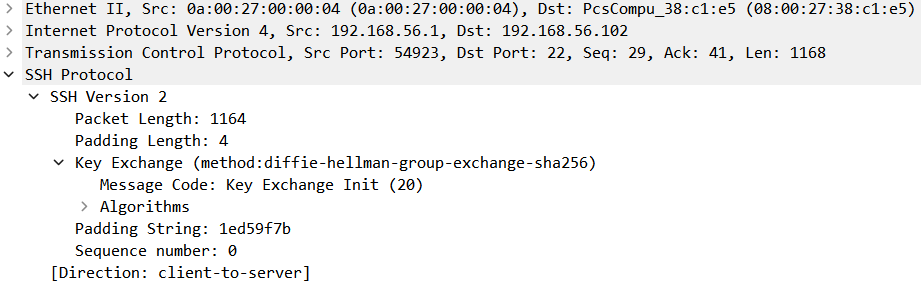
\includegraphics[scale=0.85]{images/Constitution_trames.png}
    \caption{Une trame SSH repose sur d'autres protocoles. Source : \cite{cadegros_etude_2023}}
\end{figure}

\paragraph{}
On reconnaît ici les différentes couches énumérées précédemment. \og Key Exchange\fg représente ici les données utiles de cette trame SSH.

\subsection{Hand-Shake} \label{handshake}

\paragraph{}
Nous allons maintenant détailler les échanges lors de la phase de \og Hand Shake\fg, soit la phase d'établissement de la connexion SSH. L'initialisation de cette connexion fait appel à la couche transport, et comprend \cite{cadegros_etude_2023} :

\begin{enumerate}
    \item L'échange du numéro de version du protocole
    \item L'initialisation de l'échange de clé
    \item L'échange de clé Diffie-Hellman et l'authentification du serveur
    \item La validation des algorithmes utilisés
\end{enumerate}

Ci-dessous les trames échangées correspondante:

\begin{figure}[H]
    \centering
    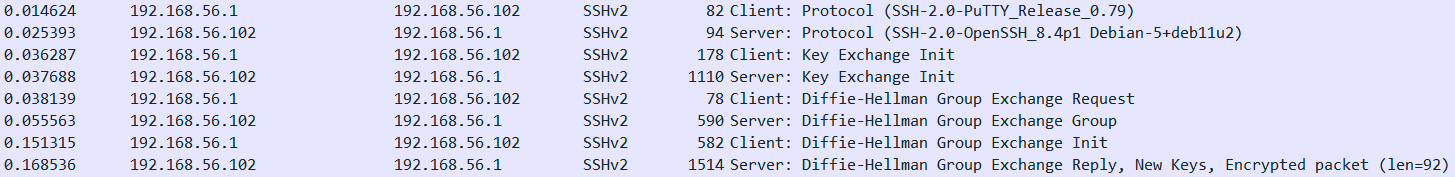
\includegraphics[scale=0.6]{images/Trames_non_chifrees.png}
    \caption{Capture des premières trames non chiffrées avec Wireshark. Source: \cite{cadegros_etude_2023}}
\end{figure}

\paragraph{Échange du numéro de version du protocole} \label{S ID C/S}
La première trame SSH envoyée par chacune des deux machines ne comporte que le numéro de version du protocole avec la version du logiciel utilisant le protocole. Cette chaîne constitue la chaîne d'identification de chacune des deux parties et sera réutilisée par la suite (cf. §\ref{ID C/S}.). L'écriture est de la forme: {\ttfamily SSH-versionprotocole-versionlogiciel commentaire CR LF}, où CR et LF représentent respectivement les caractères ASCII retour chariot et passage à la ligne.\\
Si les deux machines utilisent la version 2 de SSH, tout se passe bien. Le cas échéant, si le client utilise une version de SSH 1.X, le serveur peut parfois prendre en charge une compatibilité avec les anciennes versions. Dans ce cas, il rétrograde la version de son protocole afin de pouvoir communiquer avec le client.\\ 
Si le serveur ne prend pas en charge cette compatibilité, la connexion échoue. Si c'est le serveur qui utilise une version SSH 1.X, la connexion échoue également, et le client est invité à se reconnecter avec la même version que celle du serveur.\cite{lonvick_secure_2006}

\paragraph{Initialisation de l'échange de clé} \label{KEXINIT}
Cette étape, dont l'intitulé des trames est {\ttfamily SSH\verb|_|MSG\verb|_|KEXINIT} est cruciale à la bonne communication client-serveur, puisque chacun s'échange les algorithmes qu'il utilise pour les différentes fonctions nécessaires. Ces dernières sont la méthode d'échange de clé, l'authentification du serveur, le chiffrement, le MAC, et la compression. Ces algorithmes sont classés par catégorie, par ordre de préférence. Le client et le serveur peuvent alors deviner quel algorithme choisir. On retrouve aussi un Cookie généré aléatoirement par le serveur sur 32 octets, que le client lui renvoie, permettant d'éviter les attaques par déni de service (inonder un serveur de requête pour qu'il ne puisse plus fonctionner). \cite{hajjeh_ibrahim_protocole_2006,cadegros_etude_2023} \\

Si les deux machines ont le même algorithme d'échange de clé préféré, alors celui-ci est utilisé. Sinon, les machines regardent dans la liste du client chaque algorithme, dans l'ordre. Celui choisi sera alors le premier qui figure aussi dans la liste des algorithmes supportés par le serveur. Si aucun algorithme d'échange de clé n'est trouvé, la connexion échoue et les deux machines doivent être déconnectées.
L'algorithme d'authentification du serveur est choisi de la même manière. Cette authentification sera détaillée plus tard (cf. §\ref{Server's authentication}). \cite{lonvick_secure_2006} \\

Les algorithmes suivants nécessitant une opération différente à l'envoi et à la réception de données, chacune étant l'inverse de l'autre (on peut faire l'analogie avec une bijection réciproque en mathématiques). On retrouve deux listes pour ces fonctions. Ainsi, l'algorithme de chiffrement possède une liste pour le sens client $\rightarrow$ serveur, et une pour le sens inverse. L'algorithme choisit d'être le premier dans les deux listes du client, et doit être dans les deux listes d'algorithme du serveur. Si aucun algorithme ne répond à ces critères, la connexion échoue et les deux machines doivent se déconnecter.
Il en est de même pour les algorithmes de MAC et de chiffrement des données. \cite{lonvick_secure_2006} \\

L'échange de clé nécessite une description plus approfondie, la sous-partie suivante y est donc consacrée.